\documentclass[a4paper]{tufte-handout}
\usepackage{marvosym}
\usepackage[spanish]{babel}

\title{Sofisticación, participación y compromiso político en América Latina \thanks{Este trabajo es una versión revisada de la ponencia presentada en el VII Congreso Internacional de Comunicación Política y Estrategias de Campaña organizado por la Asociación Latinoamericana de Investigadores en Campañas Electorales (ALICE), Murcia, España, del 20 al 22 de septiembre de 2018.}
\\~\\~\\} 

\author{{\normalfont Basti\'an Gonz\'alez-Bustamante}\thanks{PRS DPhil in Politics, Department of Politics and International Relations and St Hilda's College, University of Oxford. Profesor Instructor, Departamento de Gesti\'on y Pol\'iticas P\'ublicas, Facultad de Administraci\'on y Econom\'ia, Universidad de Santiago de Chile.}}
\date{{\normalfont \normalsize \vspace{-1mm}University of Oxford} \\ {\LARGE \Letter} \href{mailto:bastian.gonzalezbustamante@politics.ox.ac.uk}{\textcolor{blue}{\normalfont \normalsize bastian.gonzalezbustamante@politics.ox.ac.uk}}
}%% \\~\\} % without \date command, current date is supplied

\hyphenation{Latino-america-na Elecci\'on eleccio-nes ALACIP}

%% \geometry{showframe} % display margins for debugging page layout

\usepackage{graphicx} % allow embedded images
  \setkeys{Gin}{width=\linewidth,totalheight=\textheight,keepaspectratio}
  \graphicspath{{graphics/}} % set of paths to search for images
\usepackage{amsmath}  % extended mathematics
\usepackage{booktabs} % book-quality tables
\usepackage{units}    % non-stacked fractions and better unit spacing
\usepackage{multicol} % multiple column layout facilities
\usepackage{lipsum}   % filler text
\usepackage{fancyvrb} % extended verbatim environments
  \fvset{fontsize=\normalsize}% default font size for fancy-verbatim environments

% Standardize command font styles and environments
\newcommand{\doccmd}[1]{\texttt{\textbackslash#1}}% command name -- adds backslash automatically
\newcommand{\docopt}[1]{\ensuremath{\langle}\textrm{\textit{#1}}\ensuremath{\rangle}}% optional command argument
\newcommand{\docarg}[1]{\textrm{\textit{#1}}}% (required) command argument
\newcommand{\docenv}[1]{\textsf{#1}}% environment name
\newcommand{\docpkg}[1]{\texttt{#1}}% package name
\newcommand{\doccls}[1]{\texttt{#1}}% document class name
\newcommand{\docclsopt}[1]{\texttt{#1}}% document class option name
\newenvironment{docspec}{\begin{quote}\noindent}{\end{quote}}% command specification environment

 \pdfinfo{
   /Author (Basti\'an Gonz\'alez-Bustamante)
   /Title  (ForceAtlas2, un algoritmo de dise\~no gr\'afico contin\'uo)
   Subject (Tufte Working Papers)
   %% /Keywords (Capital pol\'itico, elecciones, gasto en campa\~nas, incumbencia, Chile.)
}

\addto\captionsspanish{
%%\def\refname{Bibliograf\'ia consultada}
\def\tablename{Tabla}
\def\figurename{G\'rafico}
}

%% \usepackage[numbers]{natbib}
%% \usepackage{cclicenses}

\usepackage{subfig}

\usepackage{emerald}
\usepackage[T1]{fontenc}

\usepackage{multirow} 

\usepackage{hyperref}

\usepackage{xcolor, colortbl}

\usepackage{lipsum}  

\begin{document}

\maketitle

\vspace{8mm}
\justify{\small {\bfseries Resumen:} \marginnote{{\itshape {\bfseries Palabras clave:} }}}\\~\\

{\noindent \LARGE \itshape }\\

\justify{\small {\bfseries Abstract:} \marginnote{{\itshape {\bfseries Keywords:} }}}

\vspace{8mm}
\section[Introducci\'on] {{\normalfont Introducci\'on}\footnote{Agradezco al Proyecto de Opinión Pública de América Latina (LAPOP) y a sus principales donantes (la Agencia de los Estados Unidos para el Desarrollo Internacional, el Programa de las Naciones Unidas para el Desarrollo, el Banco Interamericano de Desarrollo y Vanderbilt University) por poner a disposición los datos utilizados en este trabajo. También agradezco los comentarios de Antoine Maillet. Esta investigación fue parcialmente financiada por el Convenio de Desempeño 2018 de la Universidad de Santiago de Chile.}}

\justify{La sofisticación política, también definida como conocimiento político, tiene relación con la cantidad de temas públicos que conoce un individuo, la profundidad con la cual los maneja y su capacidad para estructurar ideas sobre estos tópicos (Luskin, 1987, véase también Cohen y Zechmesiter, 2018). La sofisticación se tiende a correlacionar de forma robusta con distintas formas convencionales y no convencionales de participación política, como también con expresiones de compromiso.}

\justify{La literatura suele asociar a la participación política convencional principalmente con actividades como el sufragio, la participación en partidos políticos y en campañas electorales (Norris, 2009). La participación no convencional, por otra parte, se vincula a la política contenciosa de corte protestatario, la cual se ajusta al repertorio de acción colectiva disponible en un momento sociohistórico específico y está delimitada por estructuras de experiencias compartidas de aprendizaje basadas en la forma de organización de la acción colectiva (Tarrow, 2012; Tilly, 2006).  En este sentido, la ciencia política y la sociología han estudiado bastante, durante el último medio siglo, cuáles son los factores sociodemográficos y actitudinales que emergen como predictores de la participación política (Almond y Verba, 1980; Verba y Nie, 1972; Verba, Nie y Kim, 1978).}

\justify{Es posible identificar variables de largo (modelo de Columbia), mediano (modelo de Michigan) y corto plazo (modelo de Rochester) que afectan la percepción y predisposiciones políticas de los individuos (Arriagada, Navia y Schuster, 2010; González-Bustamante y Henríquez, 2013). Estos modelos se adecuan al caso y al contexto sociohistórico específico. Por otra parte, también existen cuerpos teóricos complementarios, por ejemplo, Bargsted et al. (2015) identifican al menos cuatro grupos de teorías para explicar específicamente la participación electoral: (a) explicaciones sociodemográficas; (b) aproximaciones basadas en la teoría de la elección racional; (c) enfoques basados en capital social; y (d) teorías asociadas a la movilización y acceso a la información. En el marco de esta diversidad teórica, generalmente se tiende a vincular los recursos sociales, como el nivel educacional y los ingresos, con la participación y el compromiso político (Corvalán y Cox, 2013; Dalton, 1988; Schlozman, Verba y Brady, 2012; Verba, Schlozman y Brady, 1995). Variables que representan estos recursos se suelen combinar con mediciones tradicionales para aproximarse al concepto operacional de sofisticación política (Cohen y Zechmeister, 2018).}

\justify{En las encuestas de opinión la sofisticación se ha medido con distintas baterías de preguntas tradicionales, principalmente a través de preguntas de conocimiento factual. Recientemente el Barómetro de las Américas 2016/17 de LAPOP ha cambiado su forma de medir conocimiento político por una aproximación más eficiente y efectiva donde es el entrevistador el que califica el nivel de conocimiento político del entrevistado. Esta nueva medición fue validada por Cohen y Zechmeister (2018) con preguntas de conocimiento factual que se mantuvieron en el cuestionario aplicado en Colombia\footnote{Las preguntas son las siguientes: GI1. ¿Cómo se llama el actual presidente de los Estados Unidos de América?; GI4. ¿Cuánto tiempo dura el período presidencial en Colombia?; y GIX4. ¿En qué continente queda Nigeria?}.}

\justify{Este trabajo, aún en desarrollo, analiza la pertinencia y consistencia de la medición de sofisticación política como predictor de participación y compromiso político con la ola del Barómetro de las Américas 2016/17 en 19 países de América Latina (N = 31.285). Se evalúan como formas de participación y compromiso político: participación electoral, en protestas, eficacia política, identificación partidaria, interés en la política y consumo de medios.}

\justify{Este documento se estructura en tres apartados. En primer lugar, en el apartado método, se ofrece información sobre los datos, variables y los modelos econométricos que se utilizan. Luego se presentan los resultados de los análisis en tres subapartados: (a) descriptivo-correlacional; (b) modelos logísticos agrupados de un nivel; y (c) modelos de efectos mixtos de dos niveles. Finalmente, se presenta un breve resumen con los principales hallazgos y futuras líneas de investigación.}

%%%%%%%%%%%%%%%%%%%%%%%%%%%%%%%%%%%%%%%%%%%%%%%%%%

\section[M\'etodo] {{\normalfont M\'etodo}}

\subsection[Datos y medición] {Datos y medición}

\justify{Se trabaja con las encuestas del Barómetro de las Américas 2016/17 de LAPOP en 19 países de América Latina (N = 31.285). A saber, Argentina (ARG: n = 1.528), Bolivia (BOL: n = 1.691), Brasil (BRA: n = 1.532), Chile (CHL: n = 1.625), Colombia (COL: n = 1.563), Costa Rica (CRI: n = 1.514), Ecuador (ECU: n = 1.545), El Salvador (SLV: n = 1.551), Guatemala (GTM: n = 1.546), Haití (HTI: n = 2.221), Honduras (HND: n = 1.560), México (MEX: n = 1.563), Nicaragua (NIC: n = 1.560), Panamá (PAN: n = 1.521), Paraguay (PRY: n = 1.528), Perú (PER: n = 2.647), República Dominicana (DOM: n = 1.518), Uruguay (URY: n = 1.514) y Venezuela (VEN: n = 1.558).}

\justify{Se utiliza la nueva variable de conocimiento político del Barómetro de las Américas 2016/17 de LAPOP como independiente y diversas variables relacionadas con formas de participación y compromiso político como variables dependientes, tal como se detalla en la tabla 1.}

\begin{table}[h]
  \centering
  \fontfamily{ppl}\selectfont
  %% \stepcounter{figure}
   \smallskip\noindent\small Tabla 1 \\ Operacionalización de variable independiente y dependientes \\~\\
  \begin{tabular}{c c c c}
    \toprule
    Código & Variable & Pregunta & Tipo \\
    \midrule
    CONOCIM & Conocimiento político & & \\
    VB2 & Participación electoral & & \\
    PROT3 & Participación en protestas & & \\
    EFF1 & Eficacia política externa & &  \\
    VB10 & Identificación partidaria & &  \\
    POL1 & Interés en la política & & \\
    GI0 & Consumo de medios & & \\
    \bottomrule
  \end{tabular}
  \\~\\ \smallskip\noindent\scriptsize Fuente: Elaboración propia con datos del Barómetro de las Américas 2016/17 por LAPOP, www.LapopSurveys.org.
  %% \caption{}
  %% \label{tab:muestra}
  %% \zsavepos{pos:normaltab}
\end{table}

\justify{La participación electoral varía dependiendo del país, por lo cual la medición va desde la participación en 2011 a 2016, dependiendo del trabajo de campo en cada país. Por ejemplo, en Nicaragua y México se preguntó sobre la participación en las últimas elecciones presidenciales de 2011 y 2012 respectivamente. En Ecuador, Honduras, Paraguay y Venezuela sobre la participación en las últimas elecciones presidenciales de 2013, mientras que en Chile sobre la participación en la primera ronda del mismo año. En otro conjunto de países se midió la participación en las últimas elecciones presidenciales de 2014: Bolivia, Brasil, Colombia, Costa Rica, El Salvador, Panamá y Uruguay. En el caso de Costa Rica, El Salvador y Uruguay se midió la participación en primera ronda, mientras que lo mismo sucedió con Argentina y Guatemala, pero en 2015. Por último, las mediciones más recientes corresponden a Haití, Perú y República Dominicana en 2016, de los cuales los dos primeros casos fueron participación en la primera ronda de las elecciones presidenciales.}

\justify{Es importante destacar que la participación electoral tiende a presentar problemas de sobre-reporte (Corvalán, Cox y Hernández, 2015). La respuesta a esta pregunta puede ser altamente sensible al falseamiento (faking) por deseabilidad social dadas las características de la situación que se desea medir (Calderón y Ximénez, 2014; Stark et al., 2001). En este caso, la deseabilidad social puede estar asociada a una connotación moral del sufragio sin importar si el sistema de votación es obligatorio o voluntario. Sin embargo, aunque la medición de este ítem presenta una alta variabilidad dados los contextos particulares de cada país, una ventaja importante es que se controlan los riesgos del sobre-reporte ya que en todos los casos se mide participación postelectoral auto-reportada y no participación preelectoral o intención futura de voto, la cual es más propensa a la deseabilidad social (Smets y van Ham, 2013).}

\justify{También se utilizan como variables de control en los modelos econométricos sexo (Q1: 0 = mujer; 1 = hombre), edad (Q2) y zona de residencia (UR: 0 = rural; 1 = urbana). Como se utilizan modelos con distribuciones binomiales hay tres variables dependientes que se deben recodificar como binarias: eficacia política, interés en la política y consumo de medios. La primera se recodifica tomando como valor positivo las tres categorías más “de acuerdo”. La variable interés por la política considera como valor positivo las categorías “mucho” y “algo”. Por último, para consumo de medios solo se considera el consumo diario.}

\subsection[Modelos econométricos] {Modelos econométricos}

\justify{Primero se estiman modelos logísticos de un nivel (Maximum Likelihood Logit Models) con un conjunto de datos agrupado que contiene a todos los países. Los modelos logísticos buscan explicar Yi como variable dependiente binaria para la observación i (Y = 0; Y = 1). Como tienen distintas probabilidades de ocurrencia se utiliza una distribución Bernoulli para modelar Yi (Cameron y Trivedi, 2010; Greene, 2012; Long y Freese, 2014).}

\justify{Se ajusta un modelo por variable dependiente utilizando la variable independiente sofisticación política y como control sexo, edad y residencia. Adicionalmente, se agregan 18 variables dummies, una por país de las muestras nacionales incorporadas al conjunto agrupado. Se utiliza el caso chileno como categoría de referencia. Se realizan pruebas con el factor de impacto de varianza (Variance Impact Factor, VIF) asimilando la distribución Bernoulli a una gaussiana para así controlar el nivel de multicolinealidad.}

\justify{Para las regresiones logísticas se utiliza un ajuste para modelos con muestras complejas con el estimador de varianza Taylor linealizado (Särndal, Swensson y Wretman, 1992; Skinner, Holt y Smith, 1989). Se consideran los estratos de la muestra (strata), las unidades primarias de muestro (PSUs) y un factor de expansión muestral o ponderador construido especialmente para realizar comparación entre países (weight1500). Para esto se sigue el esquema de ponderación y las recomendaciones técnicas de Vanderbilt University para el uso de datos del Barómetro de las Américas.}

\justify{Para obtener el factor de expansión especial se utiliza el ponderador de cada muestra nacional y se multiplica por un indicador simple compuesto por un valor estandarizado (n = 1.500) sobre el n de cada muestra nacional. Esto asegura la confiabilidad del proceso de inferencia estadística, sin embargo, un límite es que solo resulta posible evaluar la bondad de ajuste de los modelos con McKelvey y Zavoina R2 (Freese y Long, 2006; Long, 1997).}

\justify{Posteriormente, se utilizan regresiones logísticas multinivel de efectos mixtos (Mixed-effects Logistic Regressions), las cuales contienen efectos fijos y aleatorios. Esto permite una modelación con correlación intracluster donde las observaciones se ajustan porque comparten efectos de su mismo nivel o grupo (Cebolla, 2013; Demidenko, 2004; Maillet, González-Bustamante y Olivares, 2016; McCulloch, Searle y Neuhaus, 2008; Rabe-Hesketh y Skrondal, 2012).}

\justify{Se utilizan modelos de dos niveles por cada variable dependiente: donde para una serie de M clústeres independientes, en este caso las muestras nacionales, hay también un conjunto uj de efectos aleatorios (Pinheiro y Bates, 1995; Pinheiro y Chao, 2006). En el primer nivel se modela la variable de conocimiento político y las de control, mientras que en el segundo se anida a los países. Para estos modelos solo se reporta el logaritmo de verosimilitud (Log Likelihood, LL) y los valores del criterio de información de Akaike (1973) (Akaike Information Criterion, AIC), calculado como $(-2lnL + 2k) / n$, y el criterio de información bayesiano (Bayesian Information Criterion, BIC; véase Raftery, 1995), calculado con $D2 - (n - k) * ln (n)$.}

%%%%%%%%%%%%%%%%%%%%%%%%%%%%%%%%%%%%%%%%%%%%%%%%%%

\section[Resultados] {{\normalfont Resultados}}

\subsection[Análisis descriptivo y correlacional] {Análisis descriptivo y correlacional}

\justify{El gráfico 1 presenta la distribución de las categorías más elevadas (i.e., “muy alto” y “alto”) de conocimiento político para los países analizados. Se aprecia que los países con mayor sofisticación política en la región son El Salvador (51,19\%), Panamá (47,86\%) y Uruguay (46,89\%). Por el contrario, los países con los valores más bajos son Ecuador (23,37\%), México (21,50\%) y Haití (18,68\%). }

\begin{marginfigure}
  \centering
  \smallskip\noindent\small Grafo 1 \\ Distribución del conocimiento político-entrevistador, América Latina 2016/17
  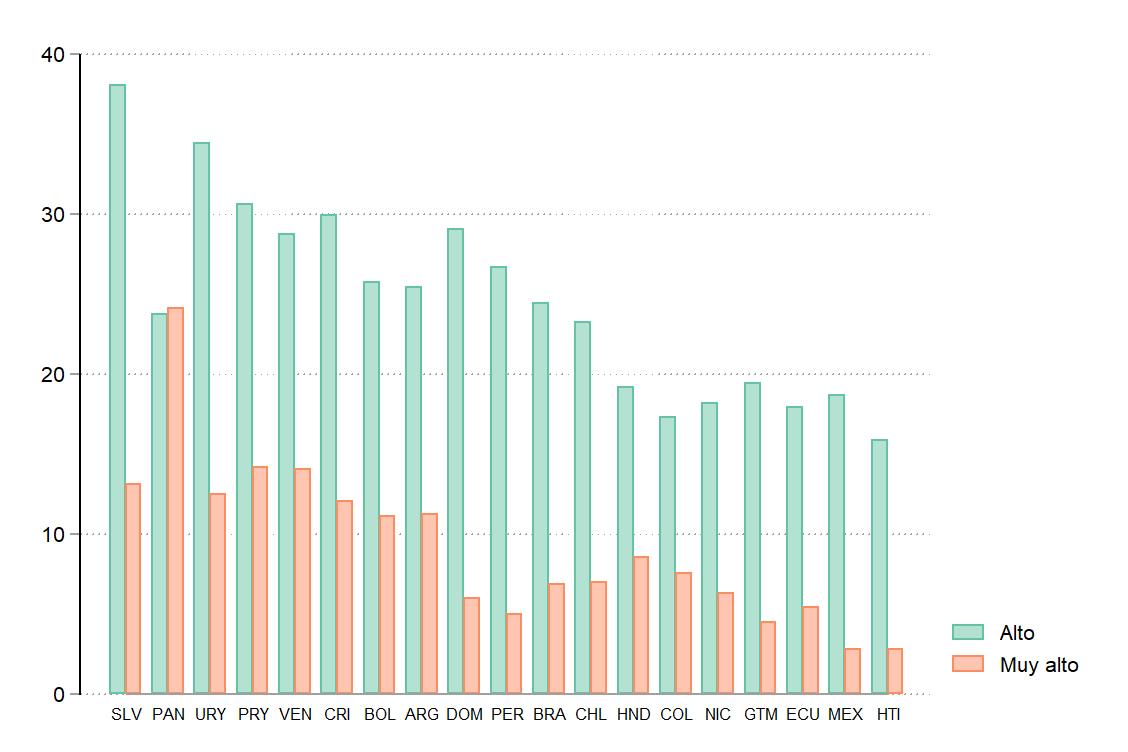
\includegraphics[width=.95\linewidth]{figures/conocim}
  %% \caption{}
  %% \label{fig:fullfig}
  \\ \smallskip\noindent\scriptsize Nota: Estimaciones puntuales ponderadas de la evaluación del conocimiento político realizada por el entrevistador. Solo se grafican las categorías “alto” y “muy alto”.\\
  Fuente: Elaboración propia con datos del Barómetro de las Américas 2016/17 por LAPOP, www.LapopSurveys.org.
\end{marginfigure}

\justify{En el gráfico 2 se puede apreciar la relación entre conocimiento político y las distintas variables dependientes con las cuales se trabaja a nivel agregado, es decir, considerando las estimaciones puntuales ponderadas de cada país. No se advierten relaciones estadísticamente significativas para participación electoral (p = 0,194), protestas (p = 0,720), eficacia política (p = 0,736) e interés en la política (p = 0,414). Se advierte una relación significativa positiva solo al 90\% entre conocimiento político e identificación partidaria: a mayor conocimiento, mayor identificación con los partidos (p = 0,074). Por último, entre conocimiento y consumo de medios se advierte una relación estadísticamente significativa, también positiva ($R^2$ ajustado = 0,274; F (1 ,17) = 7,80; p = 0,013; $\beta$ = 0,477; SD = 0,171; p = 0,013; CI95\% = 0,117; 0,837; Breusch-Pagan/Cook-Weisberg = 0,810).}

\begin{figure*}[h!]
\captionsetup[subfigure]{labelformat=empty}
  \centering
  \smallskip\noindent\small Figura 2 \\ Conocimiento político-entrevistador, participación y compromiso político, América Latina 2016/17
  \subfloat[VB2]{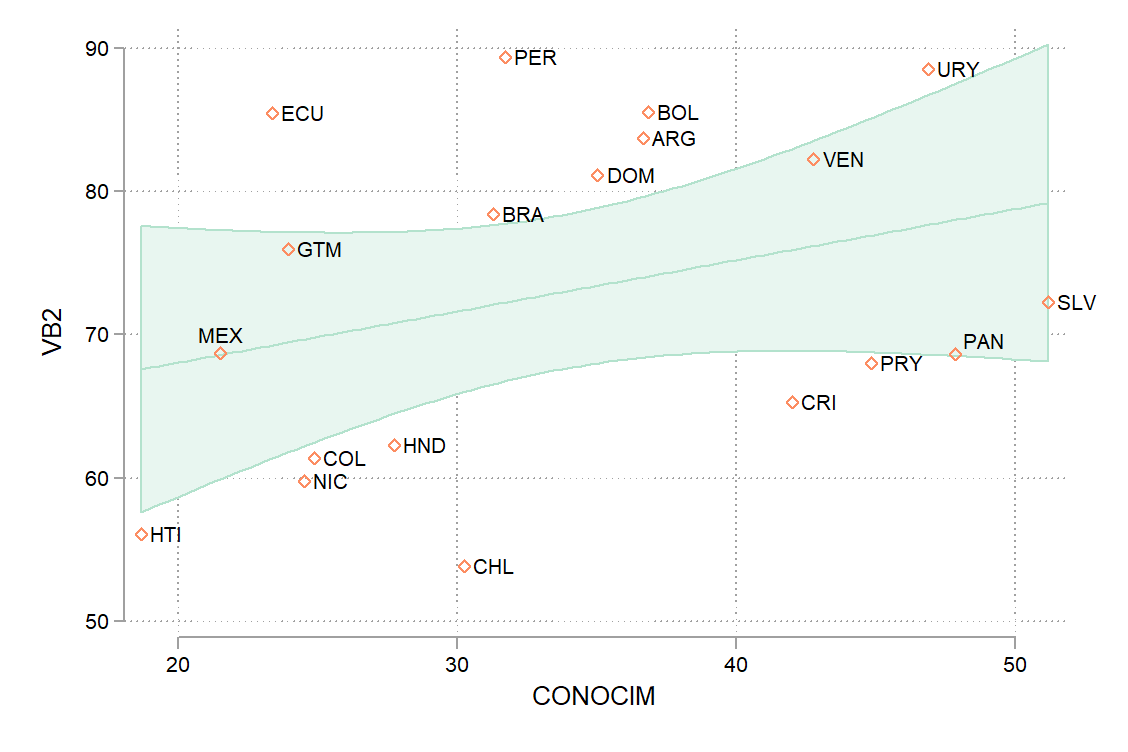
\includegraphics[width=.30\linewidth]{figures/conocim-part}}
  \subfloat[PROT3]{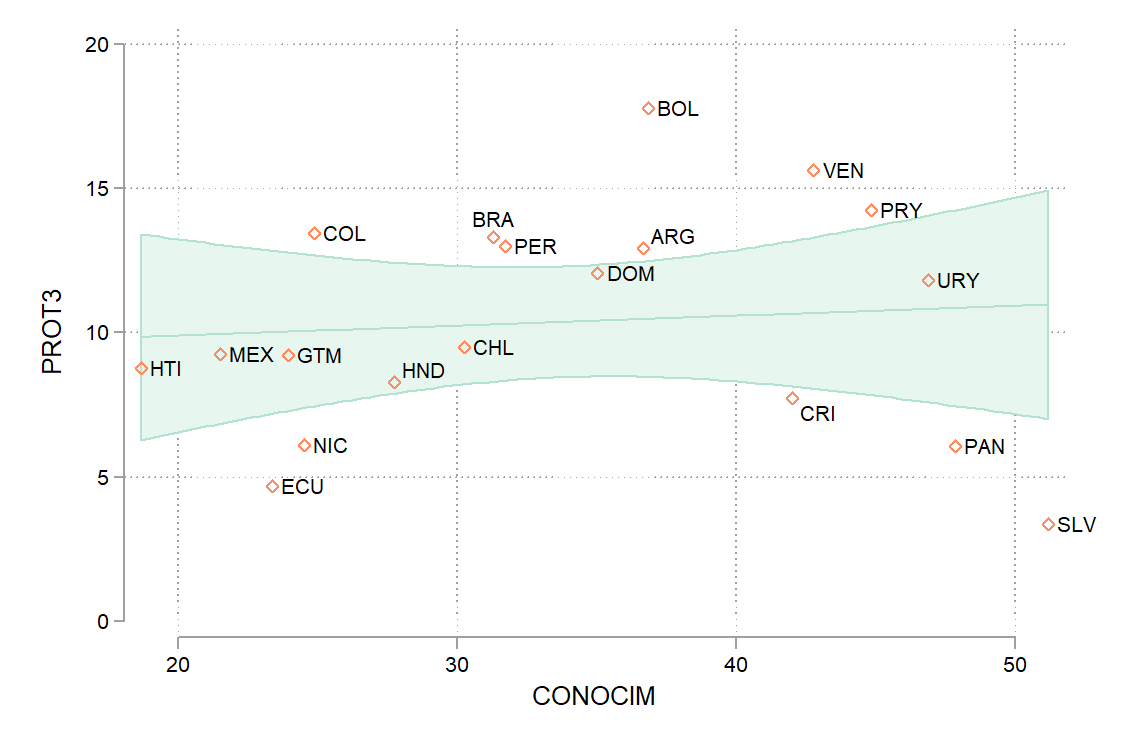
\includegraphics[width=.30\linewidth]{figures/conocim-prot}}
  \subfloat[EFF1]{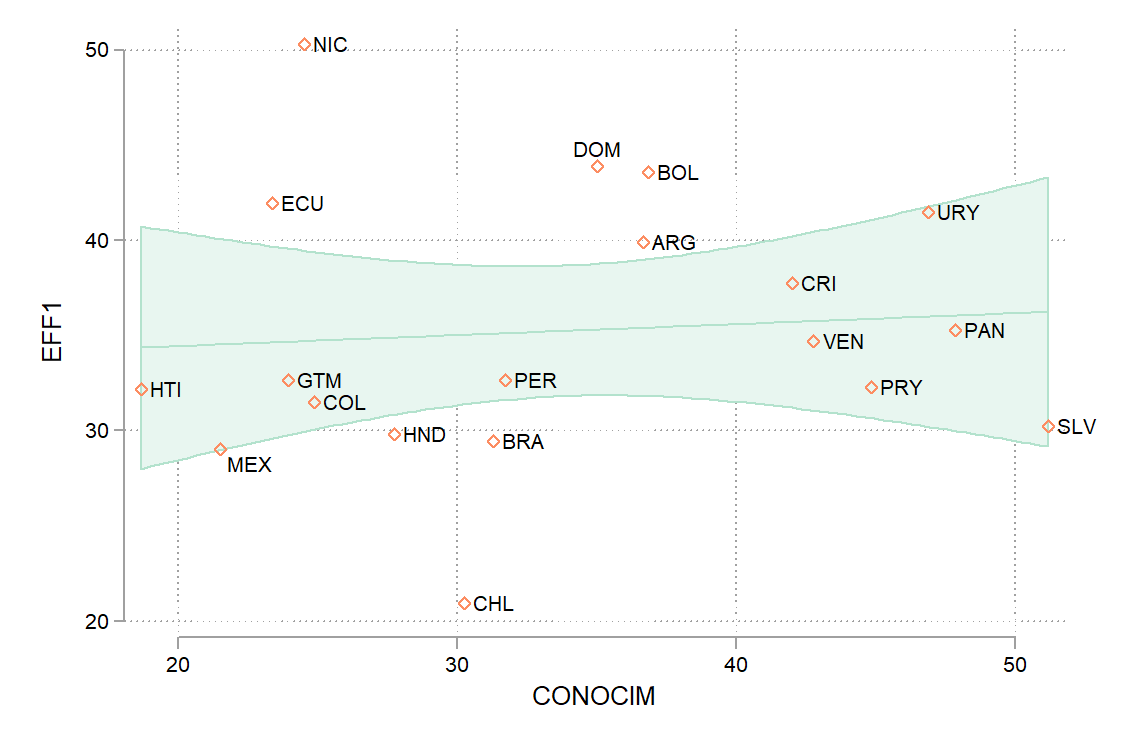
\includegraphics[width=.30\linewidth]{figures/conocim-eff}}\\
   \subfloat[VB10]{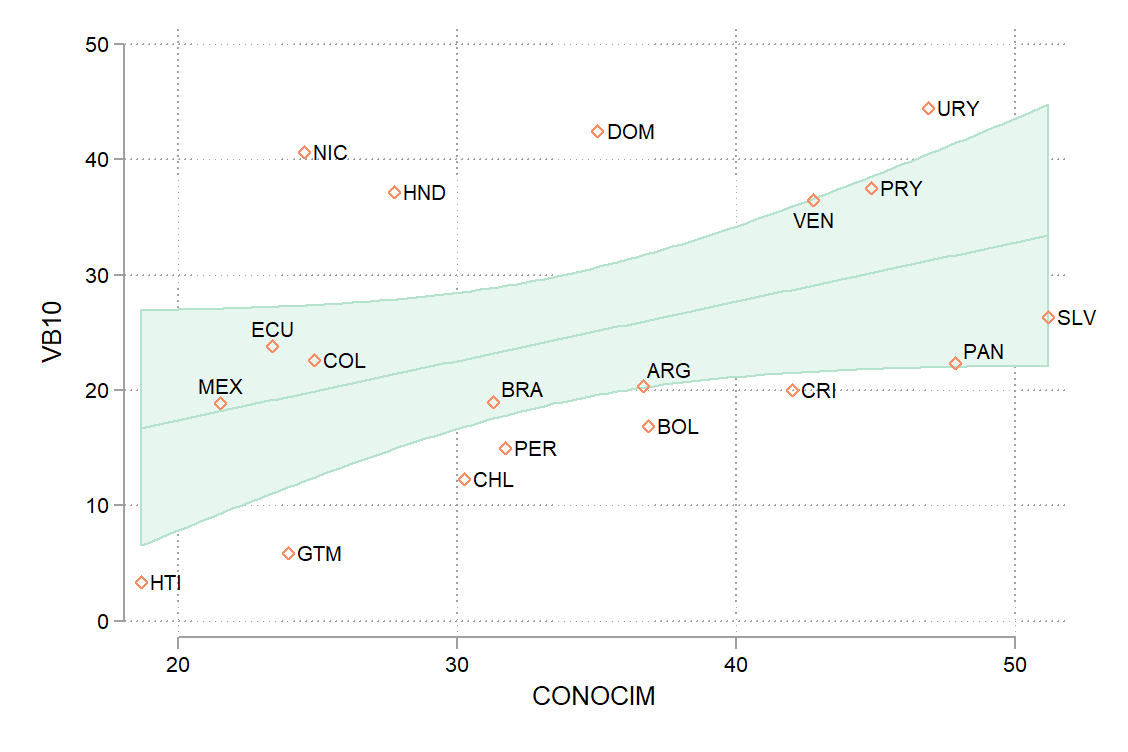
\includegraphics[width=.30\linewidth]{figures/conocim-id-part}}
   \subfloat[POL1]{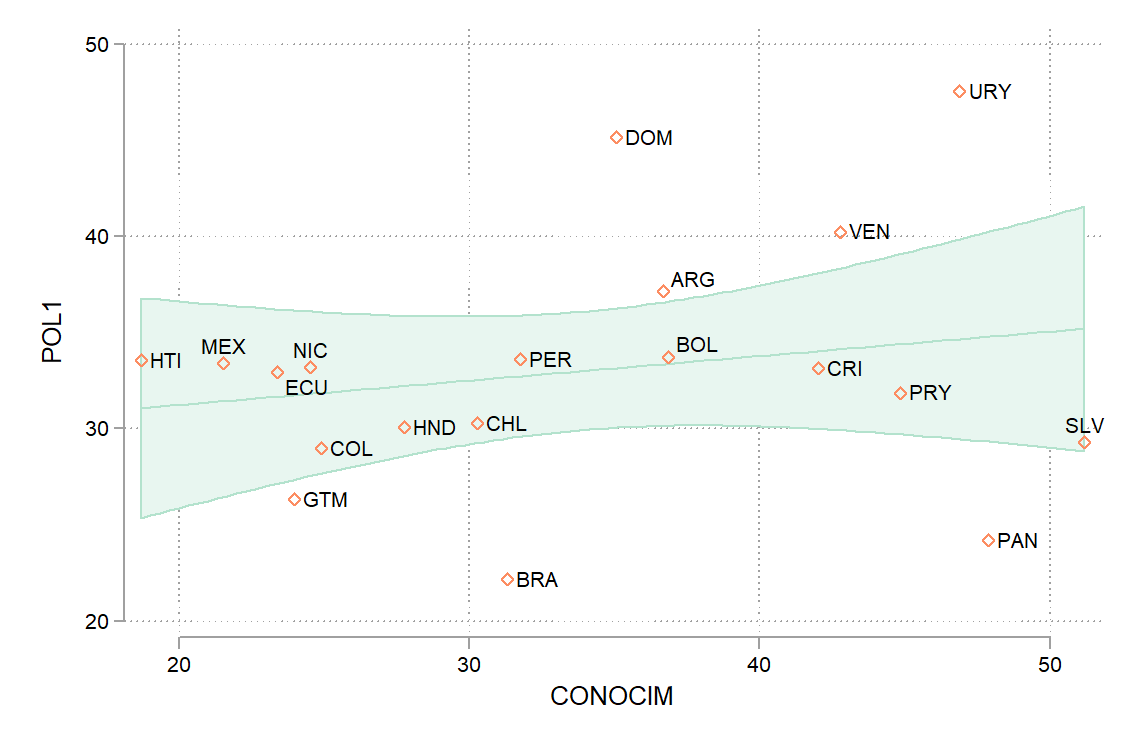
\includegraphics[width=.30\linewidth]{figures/conocim-int}}
   \subfloat[GI0]{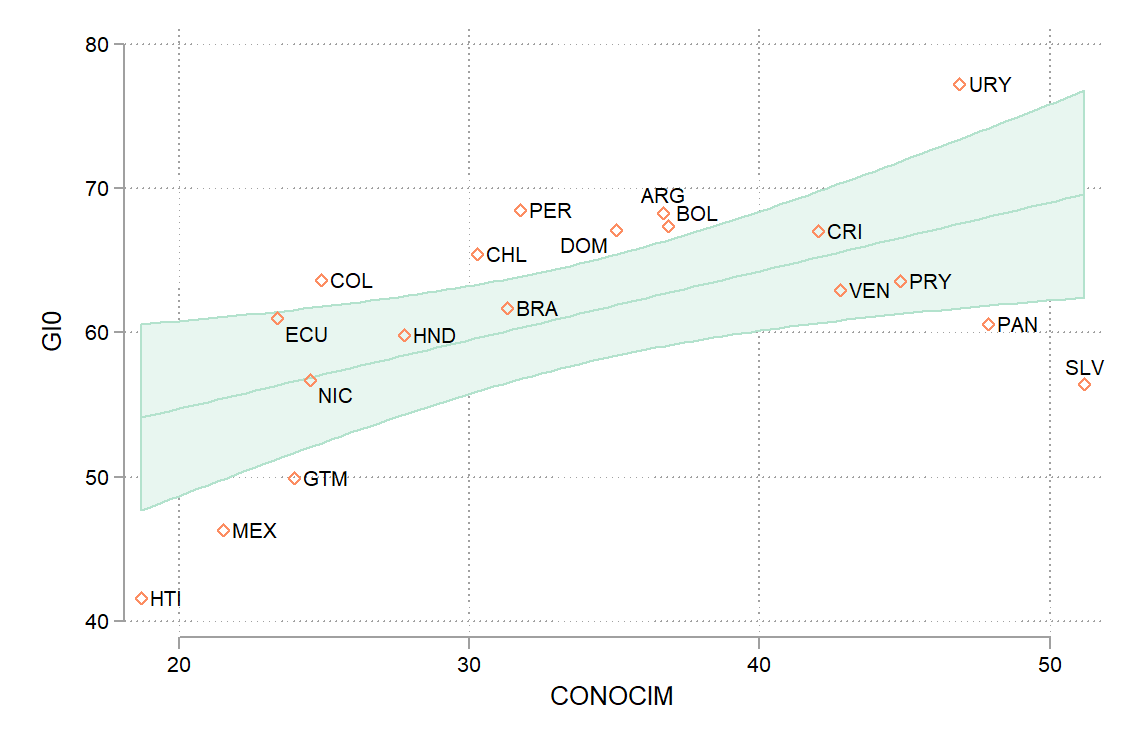
\includegraphics[width=.30\linewidth]{figures/conocim-medios}}
  %% \caption{}
  %% \label{fig:fullfig}
  \\ \smallskip\noindent\scriptsize Fuente: Elaboración propia con datos del Barómetro de las Américas 2016/17 por LAPOP, www.LapopSurveys.org.
\end{figure*}

\section[Discusi\'on] {{\normalfont Discusi\'on}}

%%%%%%%%%%%%%%%%%%%%%%%%%%%%%%%%%%%%%%%%%%%%%%%%%%

\section{{\normalfont CRediT}}

{\noindent {\bfseries Bastián González-Bustamante} (autor)}

{\noindent {
\includegraphics[width=.085\linewidth]{../../badges/conceptualization} {
\includegraphics[width=.085\linewidth]{../../badges/data_curation} {
\includegraphics[width=.085\linewidth]{../../badges/formal_analysis} {
\includegraphics[width=.085\linewidth]{../../badges/funding_acquisition} {
\includegraphics[width=.085\linewidth]{../../badges/methodology}  {
\includegraphics[width=.085\linewidth]{../../badges/computation} {
\includegraphics[width=.085\linewidth]{../../badges/testing} {
\includegraphics[width=.085\linewidth]{../../badges/data_visualization} {
\includegraphics[width=.085\linewidth]{../../badges/writing_initial_draft}
{
\includegraphics[width=.085\linewidth]{../../badges/writing_review}}\\

{\noindent {\bfseries Antoine Maillet} (comentarista)}

{\noindent {
\includegraphics[width=.085\linewidth]{../../badges/writing_review}}\\

{\noindent {\bfseries TBC} (evaluador)}

{\noindent {
\includegraphics[width=.085\linewidth]{../../badges/writing_review}}

\section{{\normalfont Referencias}}

\begin{list}{}%
{\leftmargin=1em \itemindent=-1em}

\item{\small Maillet, A., Gonz\'alez-Bustamante, B., {\itshape \&} Olivares, A. (2016). ?`Puerta giratoria? An\'alisis de la circulaci\'on p\'ublico-privada en Chile (2000-2014). {\itshape Serie de Documentos de Trabajo PNUD-Desigualdad}, (7),  1-40.}
\end{list}

\vspace{8mm}
\section[Revisión]{\LARGE \itshape Informe abierto de revisi\'on}

\vspace{8mm}
{\noindent {\Large TBC}\footnote{Biografía} \\
{\normalsize TBC} \\
\vspace{1mm}{\LARGE \Letter} \href{mailto:email@email.com}{\textcolor{blue}{\normalsize email@email.com}}}
\vspace{8mm}

\justify{\textcolor{red}{\lipsum[1]}}

\justify{\textcolor{red}{\lipsum[1]}}

\justify{\textcolor{red}{\lipsum[1]}}

\justify{\textcolor{red}{\lipsum[1]}}

%%%%%%%%%%%%%%%%%%%%%%%%%%%%%%%%%%%%%%%%%%%%%%%%%%

\end{document}
